\documentclass[journal, a4paper]{IEEEtran}

\usepackage[utf8]{inputenc}
\usepackage{cite}
\usepackage{amsmath}
\usepackage{amssymb}
\usepackage{graphicx}
\usepackage{url}
\usepackage[usenames, dvipsnames]{color}

\begin{document}

\title{Scaling of Electrode-Electrolyte Interface Model Parameters In Phosphate Buffered Saline}

\author{Mark~H.~Jones and Jonathan~Scott,~\IEEEmembership{Senior Member,~IEEE}
\thanks{Mark~H.~Jones is with the School of Electronic Engineering, University of Waikato, New Zealand, e-mail: markjones112358@gmail.com}%
\thanks{Jonathan Scott is with the School of Electronic Engineering, University of Waikato, New Zealand.}
}

\markboth{Transactions on Biomedical Circuits and Systems}
{Jones \MakeLowercase{\textit{et al.}}: Scaling of Electrode-Electrolyte Interface Model Parameters in Phosphate Buffered Saline\...}
\maketitle



\begin{abstract}
We report how the impedance presented by a platinum electrode scales with the concentration of phosphate buffered saline (PBS).
We measure the response in various dilutions of PBS with an electrode array as is commonly used in spinal cord stimulator (SCS) implants. We match the parameters of a non-linear electrode-electrolyte interface model to these measurements.
We find that the constant phase element of the model scales with approximately the log of concentration, whereas the resistivity is inversely proportional.
Using a novel DC measurement technique we show that the onset of Faradaic conduction for a platinum electrode, and thus the safe exposure limit, does not scale with concentration.
We compare objective measurements made in saline to those made in the spinal cavity of live sheep. We comment upon the appropriateness of using PBS as a substitute for in-vivo measurements.
\end{abstract}

\begin{IEEEkeywords}
    Bioelectric phenomena, Bioimpedance, Biomedical electrodes, Biomedical measurements, Biophysics, Electrical stimulation, Implantable biomedical devices
\end{IEEEkeywords}




\section{Introduction}

\IEEEPARstart{T}{here} is considerable interest in the electrical modelling of electrodes.~\cite{Cogan2008,Brown2008,Guo2012,Troy2006}
In \cite{Franks2005} a linearised model was presented, and in \cite{ScottSingle2013} a non-linear model suitable for use with the SPICE circuit simulator was presented.
The SPICE model usefully characterises an electrode in a given electrolyte with a small number of parameters.
One major reason for the interest in the electrical impedance of electrodes concerns the design of electronics intended for integration into pacemakers, cochlear implants, spinal cord stimulators, etc.
The design of successful circuits depends upon a good understanding of external load impedance, while maximisation of battery life is linked to the use of electrodes whose impedance is well understood.

Having a compact model of an electrode in the appropriate electrolyte allows circuit designers to simulate their designs with valid loads.
For example, the authors of \cite{Ethier2011} are concerned with the impedance presented by their electrode loads, and calculate power efficiency of their circuits.
This value is affected by the load impedance assumed.
Nevertheless, it is clear that they do not have a good idea of, nor a good way to simulate with, the load truly presented by an electrode in vivo or in vitro.
Knowing the effect upon the model of changes in the electrode or electrolyte would allow designers to anticipate circumstances that will affect the load seen by their circuits. 

Another appeal of a compact model stems from the fact that electrode characteristics are succinctly and objectively represented by the model parameters.
These parameters enable direct comparison of different electrodes, or the change in electrode properties over time.
For example, in \cite{Kane13} changes in chronically-implanted electrodes are observed but there is no standard quantitative way of presenting the changes.
Similarly, while there is a good understanding of what represents safe exposure, a compact model with parameters permits the prediction of the safety of any given stimulus regime.~\cite{Merrill05}

\begin{figure}
    \begin{center}
    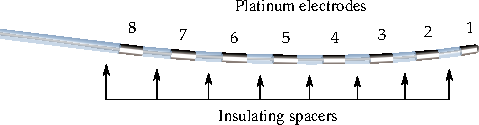
\includegraphics{graphics/StJudeOctrodeDiagram}
    \end{center}
    \caption{St. Jude Medical Octrode lead comprised of eight coaxial cylindrical platinum electrodes (1mm in diameter, 3mm long) separated by 4mm insulating spacers.}
    \label{fig:octrode}
\end{figure}

Electrodes in the laboratory are typically tested in a saline solution selected to mimic the circumstances in which they will operate when implanted.
In an implanted setting there is no reference electrode and many of the well established electrochemical measurement regimes do not apply.
Here we measure the behaviour in an electrode-electrolyte situation as it would be seen from an implant device.

The electrode used in this work is a commercial linear array of eight platinum electrodes, called an ``Octrode'', intended for Spinal Cord Stimulator (SCS) implantation.~\cite{StJudeOctrode}
A picture of an Octrode is presented in Fig.~\ref{fig:octrode}.
A solution of phosphate buffered saline (PBS) diluted to one-tenth concentration (0.1X) is commonly used as a crude phantom in the case of SCS, while full concentration (1.0X) PBS is considered more representative of the situation in blood.

Six solutions ranging from 1.0X to 0.025X the concentration (by mass) of a stock PBS solution have been examined.
The ingredients of that stock solution are given in Table~\ref{tab:PBSrecipe}.

\begin{figure}
    \begin{center}
        
\includegraphics[width=230pt]{graphics/interfaceSchematic_noMemristive}
    \end{center}
    \caption{Electrical schematic of the electrode-interface impedance model used in this work. $D_{a}$ and $D_{b}$ represent diodes; CPE and $R_{s}$ represent the constant phase element and series resistance respectively.}
    \label{fig:schematic}
\end{figure}

In this manuscript we use an adapted version of the compact non-linear model presented in \cite{ScottSingle2013}.
The model is compact in that it is suitable for entry into freely available electrical circuit simulation software.
The schematic of the electrode-electrolyte interface model that we have used is presented as Fig.~\ref{fig:schematic}.

The electrical interface models of \cite{Franks2005} and \cite{ScottSingle2013} have two parts, a displacement branch and a Faradaic branch.
Scott and Single incorporate memristors into their model, used to mimic a diffusion limited current conduction mode, i.e., their purpose is to throttle electrical current associated with Faradaic reactions.
In an implanted setting an electrode should never be operated in a Faradaic conduction mode and certainly never to the point of becoming diffusion limited; for this reason, memristors have been omitted.

It has been suggested that the primary coupling mechanism between platinum electrodes and physiological saline is the reversible evolution of gas, probably oxygen, at the platinum surface, which dissolves without bubble formation.~\cite{Greatbatch1969}
Understanding the exact mechanism of displacement or Faradaic charge transfer at the electrode surface is beyond the scope of this work.
Rather, we wish to characterise the electrode-electrolyte interface using a small number of parameters that can be fed into an electrical model.

The remainder of this manuscript is broken into five sections.
Section \ref{sect:resistorMesh} details the measurement of the inter-electrode resistances (arising from the bulk resistance of the solution) and the generation of a resistor network to replicate these resistances.
Sections \ref{sect:cpe} and \ref{sect:faradaic} are concerned with the measurement and parameter fitting of displacement currents and Faradaic currents, respectively, across the electrolyte interface.
Section \ref{sect:in-vivo} compares the results obtained for PBS with measurements made in-vivo.
Finally, in Section \ref{sect:conclusion} we summarise our findings and give concluding comments.


\section{Bulk Resistivity / Resistor Network }
\label{sect:resistorMesh}

\begin{table}
    \caption{PBS stock solution ingredients}
    \label{tab:PBSrecipe}
    \begin{center}
        \begin{tabular}{r | l}
            Ingredient & Quantity \\
            \hline
            $NaCl$ & $8.0\thinspace g$ \\
            $KCl$ & $0.2\thinspace g$ \\
            $Na_{2}HPO_{4}$ & $1.44\thinspace g$ \\
            $KH_{2}PO_{4}$ & $0.24\thinspace g$ \\
            Distilled Water & $1.0$\thinspace L \\
        \end{tabular}
    \end{center}
\end{table}

The electrical impedance between two electrodes in an electrolyte arises from two interface impedances in series with the resistance due to the bulk of the electrolyte itself.
To quantify the impedance presented by a single interface we first need to determine inter-electrode resistance presented by the electrolyte bulk.
Finding these resistances allows us to quantify the series resistance of the interface ($R_{S}$) via subtraction.
As there are always two interface impedances between any two electrodes, inter-electrode resistances cannot be measured in isolation.

In \cite{ScottSingle2013}, a series of transresistance measurements were used in conjunction with a physical description of the electrode geometry to build up a representative network of resistors.
That resistor network was defined using five parameters: $R_{eri}$, $R_{sri}$, $R_{li}$, mesh depth, and edge depth.
Readers are referred to \cite{ScottSingle2013} for the interpretation of these model parameters.
Repeating that work, we created a network of resistors that mimic the resistances due to the solution's bulk conductivity.

The mesh depth and padding values of five columns and three rows, respectively, has been taken directly from \cite{ScottSingle2013}.
These parameters, together with an array of 8 electrodes, leads to a generated network of 205 resistors, the layout of which is presented in Fig.~\ref{fig:mesh}.

A numerical fit has been made to the two independent scaling parameters $R_{eri}$ and $R_{li}$\footnote{The values of $R_{eri}$ and $R_{sri}$ are defined by the lengths of the electrode and inter-electrode spacers respectively as described in \cite{ScottSingle2013}.
The two parameters are proportional to each other by the ratio of their lengths.
Hence, we define $R_{sri}$ to be 3/4 that of $R_{eri}$ making it a dependant parameter.}.
The resulting fit and parameter values are presented in Fig.~\ref{fig:transresistance} and Table~\ref{tab:RESparams}.

Measurements of the inter-electrode impedance were made using a Tektronix TPS2014 DSO with four fully isolated and floating channels; an Agilent 33220A Function Generator; and a desktop PC running Python 2.7 for instrumentation control and result processing.
The pH level of the stock solution was measured using a calibrated EDT Instruments BA-350 pH meter.
It had a pH of 7.4 and no pH adjustments were made to the derived solutions.
The conductivity of solutions was measured using an EDT Instruments RE 388 Tx conductivity meter.

To be clear, the resistive mesh created in this step models \textit{only} the resistivity of the solution bulk.
No contribution from the interface itself appears in these measurements.
This measurement is possible because voltages are always measured across pairs of non-driven electrodes and the measurements are of suitably high impedance.
We determine the resistive component of the interface, $R_{S}$, in the following section.

\begin{figure}
    \begin{center}
        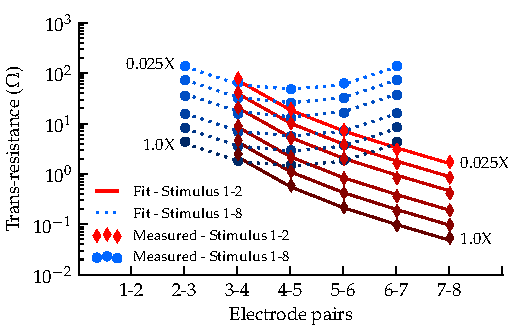
\includegraphics{graphics/pbs_transimpedance_IEEE}
    \end{center}
    \caption{Transresistance measurements (markers) used to generate the resistor mesh and the corresponding fit (lines). Red diamonds indicate results where a stimulus is placed across electrodes 1 and 2. Blue circles represent measurements where the stimulus is placed across electrodes 1 and 8. Each trace represents one of six concentrations of PBS, increasing in transresistance magnitude monotonically from 1.0X to 0.025X.}
    \label{fig:transresistance}
\end{figure}


\begin{table}
    \caption{Resistor mesh parameters. Electrolyte conductivity ($\sigma$) is expressed in units of $S / cm$}
    \label{tab:RESparams}
    \begin{center}
        \begin{tabular}{r | l}
            Parameter & Value \\
            \hline
            $R_{eri}$ ($\Omega$)& 0.407 / $\sigma$\\
            $R_{sri}$ ($\Omega$)& $R_{eri}\cdot 3/4$\\
            $R_{li}$ ($\Omega$)& 3.71 / $\sigma$ \\
            Depth (layers) & 5 \\
            Padding (layers) & 3 \\
        \end{tabular}
    \end{center}
\end{table}

\begin{figure}
    \begin{center}
        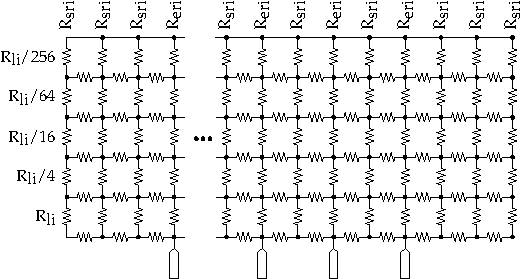
\includegraphics[width=\columnwidth]{graphics/resistorMesh_sideways}
    \end{center}
    \caption{Layout of the generated resistor mesh used to connect each of the interface models. The final mesh for an 8 electrode array contains 205 resistors.}
    \label{fig:mesh}
\end{figure}



\section{Displacement Parameters / CPE}
\label{sect:cpe}
Displacement currents are responsible for capacitive behaviour at interfacial boundaries.
They are brought about by the redistribution of charge in response to applied fields, e.g., a charged electrode will attract or repel $Cl^{-}$ from its surface and reorientate polar molecules in the surrounding solution. \cite{Merrill05}
This capacitive behaviour may also be the result of electrode polarisation in the form of reversible Faradaic reactions at the surface of the electrode.
Such reactions involving water and platinum, as identified in \cite{Horch2004,Mohtashami2011,Merrill05}, include:
\begin{eqnarray}
    Pt + H_{2}O &\Leftrightarrow& PtO + 2 H^{+} + 2 e^{-}\\
    PtO + H_{2}O &\Leftrightarrow& PtO_{2} + 2 H^{+} + 2e^{-}\\
    Pt + H^{+} & \Leftrightarrow & Pt-H\\
    Pt + H_{2}O + e^{-} &\Leftrightarrow& Pt-H+OH^{-}
\end{eqnarray}

Displacement currents are capable of transferring charge between electrical and biological systems without damaging electrodes or tissue.\cite{Horch2004}
This behaviour is modelled by way of a constant phase element (CPE), also known as a fractional capacitor.
For simulation purposes this element is realised as an array of R-C branches~\cite{ScottSingle2013,Morrison59,Elwakil10} where the value of each R-C pair is chosen to set the slope of impedance relative to frequency. The placement of R-C pairs within the CPE is determined by Morrison's parameters $m$ and $k$, where $k$ determines the spacing, or density, of R-C branches and $m$ determines the resulting slope. R-C pairs were generated using a Python script to span 1\thinspace nHz --1\thinspace GHz with a spacing of 3 pairs per decade. The CPE contains 55 branches i.e. 110 electrical elements are used to represent the CPE.


We measure displacement currents by sweeping the frequency of a sinusoidal stimulus across electrodes 2 and 7 of the Octrode while measuring the voltage between electrodes 2 and 3 (numbering shown in Fig.~\ref{fig:octrode}).
This allows for the measurement of a single interface impedance in series with the resistance presented by the bulk solution.


Current density during measurements, calculated using an effective surface area of $14\thinspace mm^{2}$, peaked at $161\thinspace \mu A/cm^{2}$ at 10\thinspace kHz in 1.0X PBS and fell as low as $197\thinspace nA/cm^{2}$ at 50\thinspace mHz in 0.025X PBS.
Charge injection per phase is shown in Fig.~\ref{fig:chargeInjectionVsFrequency} for each solution.
The stimulus waveform was set at 300\thinspace mV (peak) at each measurement point. The measurement instruments used are the same as those used to measure the inter-electrode resistance in the previous section.

\begin{figure}
    \begin{center}
        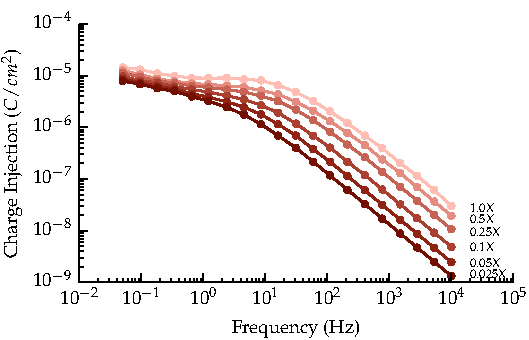
\includegraphics{graphics/chargeInjectionEffectiveVsFrequency_magnitude}
    \end{center}
    \caption{Per phase charge injected during CPE measurement in each concentrations of PBS, calculated with an effective surface area of 14\thinspace mm$^{2}$.}
    \label{fig:chargeInjectionVsFrequency}
\end{figure}


Fig.~\ref{fig:CPE_Magnitude} shows the magnitude of the measured response for each concentration of PBS accompanied by simulation results. Fig.~\ref{fig:CPE_Phase} shows the phase response for the same measurements, again with the simulated response at each concentration. The simulated responses are generated using fitted parameter values for $m$, $k$, $|Z|\thinspace @\thinspace 1Hz$, and $R_S$, which are presented in Table~\ref{tab:CPEparams}.

As shown in the interface model schematic (Fig.~\ref{fig:schematic}), the interface contains its own internal series resistance ($R_{S}$). The resistance seen in series with the CPE will therefore be the sum of both the resistance due to the bulk resistivity of the fluid and $R_{S}$, to which we will refer as $R_{S+bulk}$.
In Fig.~\ref{fig:CPE_Magnitude}, the slope and magnitude of the CPE are visible below 1\thinspace Hz whereas $R_{S+bulk}$  dominates above 1\thinspace kHz; it is clear that the two do not scale similarly.
As the impedance of the CPE and $R_{S+bulk}$ are separable with frequency, these measurements can be used to determine the CPE parameters and $R_{S}$.

Fig.~\ref{fig:CPE_Scaling} shows measured data and the corresponding fits for both the CPE magnitude at 0.05\thinspace Hz and $R_{S+bulk}$. Here we express the CPE offset parameter as $|Z|\thinspace @ \thinspace 1Hz$, but the fits used $|Z|\thinspace @ \thinspace 0.05Hz$, as data points at this frequency are outside the transitional zone where the impedance of the CPE and that of $R_{S+bulk}$ overlap.

The data presented in Fig.~\ref{fig:CPE_Magnitude} shows a large, linear, relative shift of $|Z|$ with salinity at higher frequencies, where the resistive component of the solution dominates.
Conversely, at lower frequencies where $|Z|$ changes with frequency, the relative change is closer to being logarithmic. It is this region that is modelled by the CPE.
This suggests that the CPE does not chiefly rely on the added salt ions, but they do have some effect.
Instead, the constant-phase effect must arise from phenomena not associated with the salt ions.


\begin{figure}
    \begin{center}
        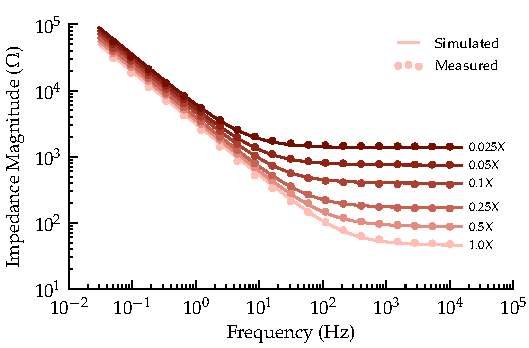
\includegraphics{graphics/displacement_impedanceVsFrequency_magnitude}
    \end{center}
    \caption{Magnitude of interfacial impedance between electrodes 2 and 7 against the frequency of a sine wave stimulus for six concentrations of PBS. The slope of the CPE is visible the left, whereas the resistance due to $R_{S+bulk}$ appears on the right. Traces represent simulated data while markers represent measured values.}
    \label{fig:CPE_Magnitude}
\end{figure}

\begin{figure}
    \begin{center}
        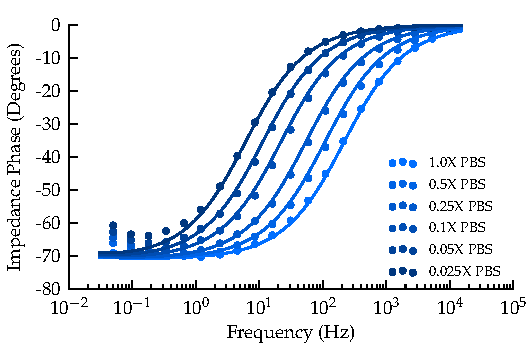
\includegraphics{graphics/displacement_impedanceVsFrequency_phase}
    \end{center}
    \caption{Phase data of interfacial impedance across electrodes 2 and 7 against frequency of a sine wave stimulus. Traces represent simulated data while markers represent measured values.}
    \label{fig:CPE_Phase}
\end{figure}

\begin{figure}
    \begin{center}
        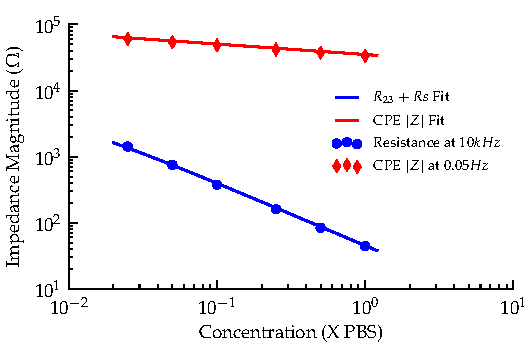
\includegraphics{graphics/scalingFactors_Displacement_IEEE}
    \end{center}
    \caption{Simulated and measured values of CPE parameters versus concentration of PBS. $|Z|$ is compared at 0.05\thinspace Hz as measured data is unaffected by $R_{S+bulk}$ at this frequency.}
    \label{fig:CPE_Scaling}
\end{figure}

\begin{table}
    \caption{Displacement parameter scaling.\hspace{\textwidth}$conc$ refers to the mass concentration of PBS.}
    \label{tab:CPEparams}
    \begin{center}
        \begin{tabular}{r | l}
            Parameter & Value \\
            \hline
            $m$ & $1.34$ \\
            $k$ & $1.773$\\
            $|Z|\: @\: 1Hz$ $(\Omega)$& $3284 \times conc^{-0.158}$ \\
            $R_{S}$ $(\Omega)$& $13.38 \times conc^{-0.8397} $\\
        \end{tabular}
    \end{center}
\end{table}



\section{Faradaic Parameters / Diodes}
\label{sect:faradaic}

With parameters fitted for the scaling of both the CPE and $R_{S}$ with PBS concentration, we turn to Faradaic conduction.
Our model uses two reverse-connected diodes to represent Faradaic current conduction between electrode and electrolyte. Specifically, we use the diodes to model irreversible Faradaic reactions. (Any reversible reactions, those producing reactants bound to the surface of the electrode, are encapsulated by the displacement branch of the model.)
Possible irreversible Faradaic reactions for platinum electrodes (each with differing reaction potentials) in saline are:

\begin{align}
    Pt + 4Cl^{-} &\Rightarrow& [PtCl_{4}]^{2-} + 2 e^{-} \label{eqn:ptCl}\\
    2H_{2}O + 2 e^{-} &\Rightarrow& H_{2}\uparrow + 2OH^{-} \label{eqn:H20}\\
    2H_{2}O &\Rightarrow& O_{2}\uparrow + 4H^{+} + 4e^{-} \label{eqn:2H20}\\
    2Cl^{-} &\Rightarrow& Cl_{2}\uparrow + 2e^{-} \label{eqn:Cl} \\
    Cl^{-} + H_{2}O &\Rightarrow& ClO^{-} + 2H^{+} + 2e^{-} \label{eqn:ClH20}
\end{align}

We use a diode to model the electrical current conduction caused by one reaction proceeding in one direction, i.e. a diode is the circuit representation of the Butler-Volmer equation for a single reaction proceeding in a single direction. 
    We wish to model the onset of Faradaic current as a way of knowing that an electrode has been pushed ``too far''. It is expected that the situation in-vivo will be much more complex and that fitted diode parameters may encapsulate multiple reactions if they occur close together.

To measure Faradaic conduction we must separate its contribution from any displacement behaviour. By using a DC measurement technique, as opposed to cyclic measurements, we are able to separate the effects in time.
Like a conventional capacitor, the CPE responds to a change in voltage by absorbing or ejecting charge, causing a spike in current. The CPE will draw negligible current once it has settled and in the case of our model we assume the remaining current conduction to be the result of Faradaic processes.

The equation governing current conduction in a diode where the forward voltage across the diode, $V_{D}$, is small is
\begin{equation}
    I = i_{0}  e^{V_{D} / n V_{T}}
\end{equation}
where $V_{T}$ is the thermal voltage and is approximately 25\thinspace mV at a temperature of 300\thinspace K. We wish to find how the saturation current ($i_{0}$) and the ideality factor ($n$) scale as the solution salinity is varied.

Faradaic measurements were made using an Agilent E5270B Precision Measurement Mainframe producing a stepped DC voltage stimulus whilst continuously measuring the output current.

Measurements commenced with a 4.5 litre solution of 1.0X PBS which was progressively diluted in factors of two between measurements. The solution was mixed continuously using a standard laboratory grade magnetic stirrer. The solution was in equilibrium with air prior to and during measurement and the electrodes remained submerged at all times.
A single measurement run involved stepping the voltage across the electrodes from 0.5\thinspace V to 1.2\thinspace V in increments of 0.05\thinspace V; this range was previously determined to capture the onset of Faradaic conduction.

In \cite{Greatbatch1969} it is shown that the stirring of an air-saturated solution of physiological saline reduces the settling time of platinum electrodes to stimulus transients; with both situations eventually settling to the same impedance.

In \cite{Cogan2008} it has been noted that results obtained using cyclic voltammetry are dependant on, among other factors, the measurement sweep rate. This indicates a lack of isolation between displacement and Faradaic mechanisms. Our measurements were repeated using wait-times of 4, 16, 32 and 64 seconds between voltage increments, allowing us to determine the effect of sweep rate. From these measurements and those of a separate investigation\footnote{We took measurements of the interface's response to voltage steps when left to settle for 10 000 seconds, of which the first 250\thinspace seconds are shown in Fig.~\ref{fig:CPE_currentVsTime}. Those measurements show a trend of decreasing current stabilisation time as the overpotential steps increase. Sixty four seconds after stepping from 0.64\thinspace V to 0.72\thinspace V, the current has stabilised to $95\%$ of its value at 10\,000 seconds. At overpotential steps for higher voltages, the settling time is further reduced. These measurements were made in still solution and we expect stirring will further reduce settling time.} we concluded that a wait-time of 64 seconds is sufficient.

\begin{figure}
    \begin{center}
        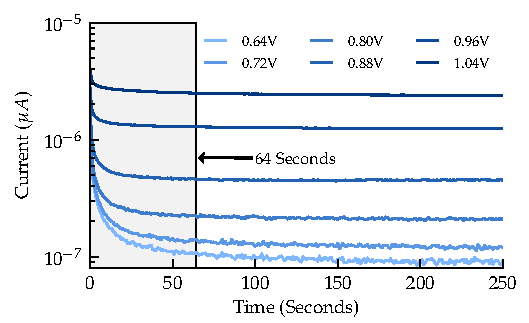
\includegraphics{graphics/CPE_currentVsTime}
    \end{center}
    \caption{Current versus time after a stepped voltage increment across a pair of interfaces. Time before 64 seconds is highlighted in grey. Measurements were taken with a wait time of 10,000 seconds between increments.}
    \label{fig:CPE_currentVsTime}
\end{figure}

In Fig.~\ref{fig:StepResponse_Faradaic}, electrical current measurements (solid lines) are plotted against time. Each spike marks the point at which the voltage is incremented by 50\thinspace mV. Note that the amount of charge absorbed by the CPE increases with concentration of PBS, but the current for each concentration converges to approximately the same value. Dotted lines have been added that link the electrical current measurements taken 10 seconds after each increment for 0.125X PBS (lower trace) and 1.0X PBS (upper trace). These dotted traces show results typical of cyclic measurement methods, where the electrode overpotential is never constant. This illustrates the benefit of using DC measurements when measuring Faradaic currents.

Fig.~\ref{fig:faradaic_logCurrentVsVoltage} shows the settled currents plotted on a log scale, versus the voltage applied across the electrode pair. This uses the same data as the previous figure but has been processed so that each point represents the average of the final 24 current measurements at each step. Below 0.9\thinspace V it appears that the concentration of the solution had no identifiable effect on Faradaic conduction as there is overlap between each trace and the mean values are not monotonic with concentration in this region.  Between 0.9\thinspace V and 1.05\thinspace V a transition occurs which results in current conduction becoming dependent on solution concentration.
Above 1.05\thinspace V the traces diverge showing clear dependence upon concentration.
The point at which this transition occurs is determined by the concentration of saline, with lower concentrations transitioning earlier. A concentration of 0.0625X PBS causes a transition at around 0.95\thinspace V whereas electrodes in the 1.0X PBS solution transition somewhere between 1.0\thinspace V and 1.05\thinspace V. The effect of transition can be seen in the green trace at 1.0\thinspace V where the error bar is wide due to the current shift being captured in the measurement at that voltage. Part of a transition with respect to time is visible in Fig.~\ref{fig:StepResponse_Faradaic} where the red trace drops uncharacteristically after the increment at around 600 seconds.

\begin{figure}
    \begin{center}
        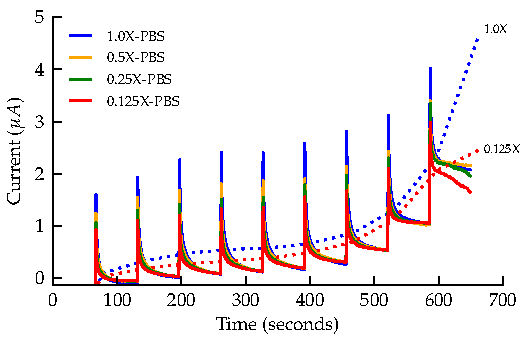
\includegraphics{graphics/currentTimeFaradaicCPE_Stacked_IEEE}
    \end{center}
    \caption{Current conduction with 0.05\thinspace V stepped voltage increments from 0.5\thinspace V to 0.9V. Each voltage is held for 64 seconds before being further incremented. Dotted lines connect current measurements occurring 10 seconds after an increment.}
    \label{fig:StepResponse_Faradaic}
\end{figure}


\begin{figure}
    \begin{center}
        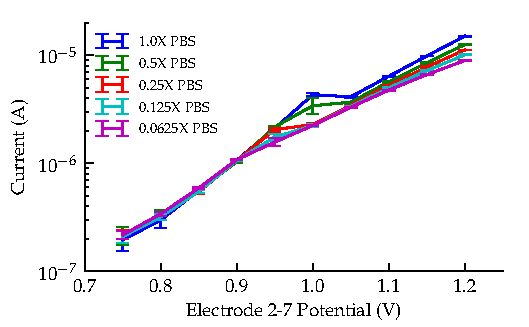
\includegraphics{graphics/currentVoltage_logY_IEEE}
    \end{center}
    \caption{Faradaic conduction as a function of voltage applied across electrodes 2 and 7. Samples shown were taken between 40 and 64 seconds after each voltage increment. Error bars indicate spread in measurement results, where 95\% of samples lie within the bars.}
    \label{fig:faradaic_logCurrentVsVoltage}
\end{figure}

\begin{figure}
    \begin{center}
        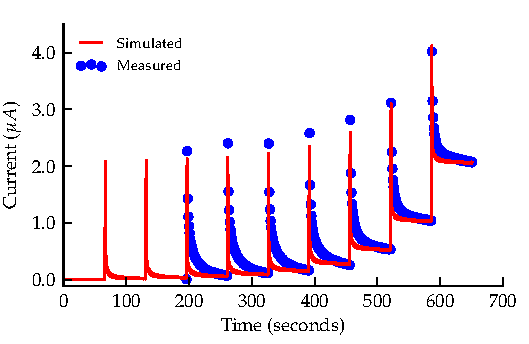
\includegraphics{graphics/faradaic_currentVsTimeIEEE}
    \end{center}
    \caption{Current versus time for 1.0X PBS overlaid with simulated results of the interface model's response to increasing voltage steps. The model used for simulation includes the CPE, diodes and $R_{S}$.}
    \label{fig:faradaic_currentVsTime}
\end{figure}

\begin{figure}
    \begin{center}
        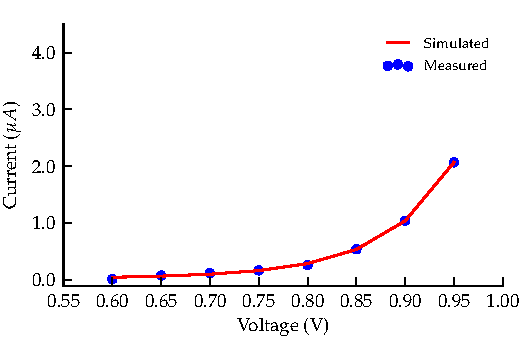
\includegraphics{graphics/faradaic_currentVsVoltageIEEE}
    \end{center}
    \caption{Simulated response of the interface model compared to measurement from the electrodes with a stepped voltage overpotential. Measurement points show current values taken at the $64^{th}$ second after each voltage increment.}
    \label{fig:faradaic_currentVsVoltage}
\end{figure}

\begin{table}
    \caption{Faradaic parameters}
    \label{tab:FaradaicParams}
    \begin{center}
        \begin{tabular}{r | l}
            Parameter & Value \\
            \hline
            $i0$ & $2.757\thinspace pA$\\
            $n$ & 1.36\\
        \end{tabular}
    \end{center}
\end{table}

We attribute the change in behaviour between 0.9\thinspace V and 1.05\thinspace V to a transition to diffusion-controlled conduction.
We hypothesise that the charging of the CPE draws available ions to the electrode, creating a layer of high ionic concentration at the surface irrespective of that of the solution bulk. It is this layer that is subsequently consumed by the Faradaic reactions at a rate that increases exponentially with electrode overpotential.  The effect of bulk solution concentration while this layer has formed is negligible until the point at which the layer is consumed faster than it can be replenished. At this stage, and with increasing overpotential, the Faradaic conduction is governed by diffusion of ions from the bulk into the layer, the rate of which increases with the ion concentration in the bulk. We believe this explains the divergence of conduction with concentration between 0.9\thinspace V and 1.05\thinspace V and why there is no observable dependence on bulk ion concentration beforehand.
For the purposes of our model, we are content with placing a limit of 0.9\thinspace V across the pair of interfaces and using the assumption that Faradaic conduction does not change with concentration. As we are primarily interested with capturing only the onset of Faradaic conduction, this limitation does not degrade the usefulness of the model for implant modelling purposes.


    Fig.~\ref{fig:faradaic_currentVsTime} shows a subset of the data used in Fig.~\ref{fig:StepResponse_Faradaic} (the 1.0X PBS trace) to show the fit between simulated and measured data in the time domain. Here the simulation contains fitted diode parameters, shown in Table~\ref{tab:FaradaicParams}, which give rise to the exponentially increasing steady state current.
It is apparent from this trace that the temporal response of the CPE does not match the transient decay curves seen in the Faradaic measurements, something the CPE should predict. These transient decay curves appear to have a time-constant\footnote{We use the term ``time-constant'' although a CPE does not have a simple exponential time-domain response.} that decreases with each subsequent measurement. This variable time-constant phenomena is especially clear when looking at Fig.~\ref{fig:CPE_currentVsTime}. Although the Faradaic response transients appear to approach the time-constant predicted by the CPE, there is still behaviour not completely described by the CPE.

The match between fitted diode parameters ($n$ and $i_{0}$) and the measurement data 64 seconds after each voltage increment has been plotted in Fig.~\ref{fig:faradaic_currentVsVoltage}.

In future we hope to extend this model into a diffusion controlled conduction scenario and extend the CPE element to better reproduce the time domain response.


\section{In-vivo measurements of sheep}
\label{sect:in-vivo}
\begin{figure}
    \begin{center}
        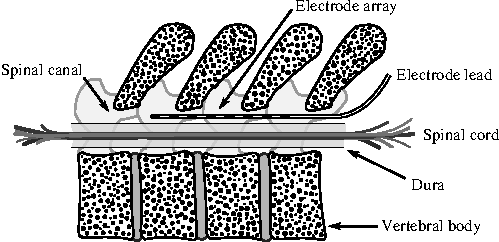
\includegraphics{graphics/sheepSpine}
    \end{center}
    \caption{Cross section of a sheep spine showing the position of the electrode array relative to the dura. Spotted regions represent cross sectioned vertebrae.}
    \label{fig:sheepSpine}
\end{figure}

\begin{table}
    \caption{Model parameters fitted to sheep data}
    \label{tab:sheepParameters}
    \begin{center}
        \begin{tabular}{r | l}
            Parameter & Value \\
            \hline
            $R_{eri}$ & $500\thinspace \Omega$\\
            $R_{sri}$ & $375\thinspace \Omega$\\
            $R_{li}$  & $176\thinspace \Omega$\\
            $m$       & $1.34$\\
            $k$       & $1.77$\\
            $|Z|\: @\: 1Hz$& $11300\thinspace \Omega$\\
            $R_{s}$   & $126\thinspace \Omega$
        \end{tabular}
    \end{center}
\end{table}

\begin{figure}
    \begin{center}
        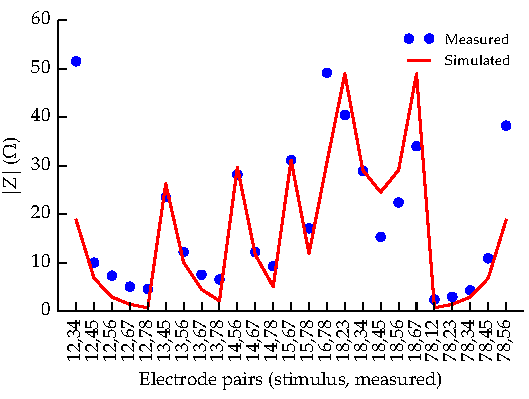
\includegraphics{graphics/sheep_transimpedance_doubleFit_mag}
    \end{center}
    \caption{Comparison between the magnitude of in-vivo transresistance measurements (blue dots) and simulation results using fitted mesh parameters (red trace).}
    \label{fig:transimpedance_sheep_mag}
\end{figure}

\begin{figure}
    \begin{center}
        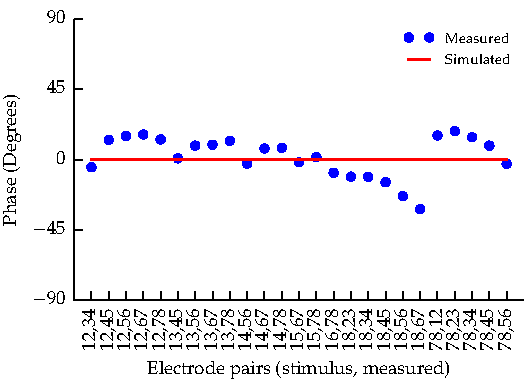
\includegraphics{graphics/sheep_transimpedance_doubleFit_phase}
    \end{center}
    \caption{Comparison between the phase of in-vivo transresistance measurements (blue dots) and simulation results using fitted mesh parameters (red trace). The simulation mesh does not capture any phase relationship due to being purely resistive.}
    \label{fig:transimpedance_sheep_phase}
\end{figure}

Cogan states the main differences between in-vivo and in-vitro responses come down to temperature, the presence of organic species, tortuous diffusion path for charge carriers, physiological responses of the host to a foreign body, and uncertain concentrations of electrolytes and buffers near the electrode surface.\cite{Cogan2008}
Nevertheless, electrical engineers use baths of saline as a substitute for in-vivo testing (a ``phantom'') due to its convenience.
We now test the claim that 0.1X PBS is a reasonable representation of the spine of a living sheep.

Each of the model characterisation measurements were repeated inside the spinal canal of living sheep, just outside the dura as shown in Fig.~\ref{fig:sheepSpine}. Two sheep were prepared and anaesthetised using the procedures described in \cite{Parker2013} under the Animal Care and Ethics Committee approval of the Royal North Shore Hospital, Sydney. The study complied with the Australian Code of Practice for the Care and Use of Animals for Scientific Purposes.

Transimpedance measurements in-vivo were conducted with additional configurations than were carried out in Section \ref{sect:resistorMesh}. The same measurements were captured except this time using a larger number of stimulus--measure configurations in order to minimise the effect of nearby bone. Time constraints with the live animal meant only a single dataset was obtained for transimpedance. This data is shown in Figs.~\ref{fig:displacement_sheepCPEMagnitude} and \ref{fig:displacement_sheepCPEPhase} along with results obtained from simulation with fitted parameters.

In these measurements a phase deviation of approximately 30 degrees is observed, visible in Fig.~\ref{fig:transimpedance_sheep_phase}. There was no measurable phase deviation for these measurements in PBS. These results indicate that the sheep itself presents a significant reactive component.

Four measurements of displacement current (CPE element in the model) were taken at regular intervals over a period of 30 minutes, the mean response is presented in Figs.~\ref{fig:displacement_sheepCPEMagnitude} and~\ref{fig:displacement_sheepCPEPhase}.
These measurements appear on top of the traces taken from Figs.~\ref{fig:CPE_Magnitude} and~\ref{fig:CPE_Phase} for comparison.

Although it is clear that there are complications in vivo, a 0.25X PBS solution offers a good approximation to the resistive part of the  trace.
The reactive part (that of the CPE) would be better modelled by a solution of less than 0.025X concentration.  

Faradaic measurements on the live animal were abandoned as they were likely to cause potentially violent muscle contraction. Attempts to measure the response at low stimulus potentials yielded unsatisfactory results and were subsequently discarded. 

\begin{figure}
    \begin{center}
        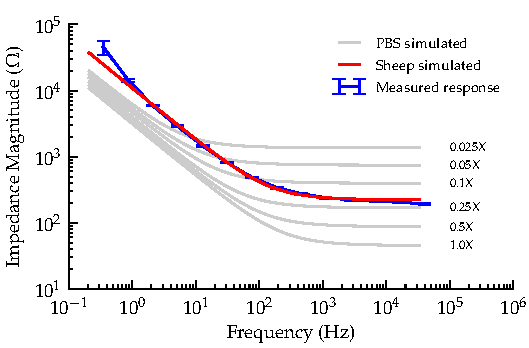
\includegraphics{graphics/displacement-withSheep_impedanceVsFrequency_magnitude}
    \end{center}
    \caption{Comparison between the mean magnitude of measured displacement currents in four live sheep (blue trace), each of the PBS traces from Fig.~\ref{fig:CPE_Magnitude} (grey lines), and a simulated fit to the sheep data (red trace). Error bars have been placed one standard deviation either side of the mean for measured data.}
    \label{fig:displacement_sheepCPEMagnitude}
\end{figure}

\begin{figure}
    \begin{center}
        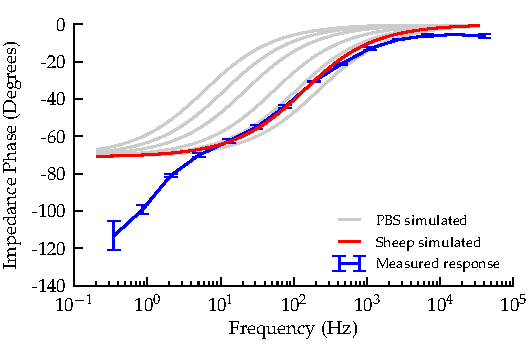
\includegraphics{graphics/displacement-withSheep_impedanceVsFrequency_phase}
    \end{center}
    \caption{Comparison of the mean phase response of measured displacement currents in live sheep (blue trace), each of the PBS traces taken from Fig.~\ref{fig:CPE_Phase} (grey lines), and a simulated fit to the sheep data (red trace). Error bars have been placed one standard deviation either side of the mean for measured data.}
    \label{fig:displacement_sheepCPEPhase}
\end{figure}





\section{Conclusion}
\label{sect:conclusion}
We have used the parameters of a compact electrical model of an implantable electrode as a way of objectively comparing scenarios.
We have measured how changing the concentration of PBS affects the parameters of this model.
We have drawn direct relationships with concentration and conductivity sufficient to predict interface characteristics at arbitrary dilutions of PBS.
We found that the magnitude of the CPE element moves much more slowly with concentration whereas the resistance moved almost linearly.
Using DC measurements we conclude that the concentration of PBS has no effect on the onset of Faradaic conduction for the range of concentrations measured.
We hypothesise that this is because the double-layer sets the concentration of species involved in the Faradaic reactions within a volume surrounding each electrode.

In-vivo measurements using platinum electrodes in sheep spine show that no single concentration of PBS matches both the CPE and the resistive characteristics at once.
These measurements also reveal a considerable amount of reactance (see transimpedance measurements in vivo) that is captured neither by PBS nor the model presented when using a purely resistive spreading resistance.
Nevertheless, if a single solution of PBS is to be used as a human phantom, a one-tenth concentration solution (by mass) is a good compromise.

While the model used is limited to predicting only the onset of Faradaic current conduction, it usefully captures the transition into this biologically destructive stimulus regime sufficient for it to be avoided. 
    
The final model, including 205 lines of resistive mesh, is represented by a SPICE netlist comprised of 348 lines.
A simulation of this model, using the freely available ngSpice circuit simulator, at 1000 frequencies takes approximately 1 second on a modern CPU.

\section*{Acknowledgement}
The authors acknowledge The University of Waikato for financial support and Saluda Medical for the use of facilities and equipment. Special thanks are expressed to Peter Single of Saluda Medical for help conducting in-vivo measurements and to the anonymous reviewer whose detailed comments lead to a much more rigorous manuscript.

\begin{thebibliography}{99}


\bibitem{Cogan2008}
    Stuart~F.~Cogan,
    ``Neural Stimulation and Recording Electrodes'',
    Annu. Rev. Biomed. Eng. 2008. pp275--309.

\bibitem{Troy2006}
    John~B.~Troy, Donald~R.~Cantrell, Allen~Taflove and Rodney~S.~Ruoff
    ``Modeling the electrode-electrolyte interface for recording and stimulating electrodes'',
    {\em Proceedings of the 28th IEEE EMBS Annual International Conference}
    New York City, USA, Aug. 30, 2006, pp879--881.

\bibitem{Brown2008}
    Edgar~A.~Brown, James~D.~Ross, Richard~A.~Blum, Yoonkey~Nam, Bruce~C.~Wheeler and Stephen~P.~DeWeerth,
    ``Stimulus-Artifact Elimination in a Multi-Electrode System'',
    {\em IEEE Transactions on Biomedical Circuits and Systems},
    vol.~2 no.~1, March 2008, pp10--21.

\bibitem{Guo2012}
    Jing~Guo, Jie~Yuan and Mansun~Chan,
    {\em IEEE Transactions on Biomedical Circuits and Systems},
    vol.~6 no.~6, December 2012, pp605--613.

\bibitem{Franks2005}
    W.~Franks, Iwan~Schenker, Patrik~Schmutz, and Andreas Hierlemann,
    ``Impedance Characterization and Modeling of Electrodes for Biomedical Applications'',
    \emph{IEEE Transactions on Biomedical Engineering},
    vol.~52 no.~7, July 2005, pp1295--1302.

\bibitem{ScottSingle2013}
    Jonathan Scott and Peter Single,
    ``Compact Nonlinear Model of an Implantable Electrode Array for Spinal Cord Stimulation (SCS)'',
    to be published in
    \emph{IEEE Transactions on Biomedical Circuits and Systems},
    DOI: 10.1109/TBCAS.2013.2270179, 2013.

\bibitem{Ethier2011}
    Sébastien Ethier and Mohamad Sawan,
    ``Exponential Current Pulse Generation for Efficient Very High-Impedance Multisite Stimulation'',
    \emph{IEEE Transactions on Biomedical Circuits and Systems},
    vol.~5 no.~1, February 2011, pp30--38.


\bibitem{Kane13}
    Sheryl~R.~Kane, Stuart~F.~Cogan, Julia~Ehrlich, Timothy~D.~Plante, Douglas~B.~McCreery and Philip~R.~Troyk,
    ``Electrical Performance of Penetrating Microelectrodes Chronically Implanted in Cat Cortex``,
    {\em IEEE Transactions on Biomedical Engineering},
    vol.~60 no.~8, August 2013, pp2153--2160.

\bibitem{Merrill05}
    Daniel~R.~Merrill, Maron Bikson and John~G.~R.\ Jefferys,
    ``Electrical stimulation of excitable tissue: design of efficacious and safe protocols'',
    Journal of Neuroscience Methods 141 (2005), pp171--198.

\bibitem{StJudeOctrode}
    St.~Jude Medical, Octrode Percutaneous Lead for Neuromodulation,
    \url{http://www.sjmneuropro.com/Products/US/Percutaneous-Leads.aspx},
    retrieved December 2012.

\bibitem{Greatbatch1969}
    W.~Greatbatch, B.~Piersma, F.~D.~Shannon, and S.W.~Calhoon, S. W.
    ``Polarization phenomena relating to physiological electrodes'',
    Annals of the New York Academy of Sciences,
    167(2), 1969 pp722-744.


\bibitem{Mohtashami2011}
    Saba~Mohtashami,
    ``Electrochemical Properties of Flexible Electrodes for Implanted Neuromuscular Excitation Applications'',
    Open Acess Dissertations and Theses (2011), Paper 6152

\bibitem{Horch2004}
    K.~W.~Horsch and G.~S.~Gurpreet,
    ``Neuroprosthetics: theory and practice'',
    World Scientific, 2004.

 \bibitem{Morrison59}
    Ralph Morrison,
    ``RC Constant-Argument Driving-Point Admittances'',
    {\em IRE Transactions on Circuit Theory},
    September 1959, pp310--317.

\bibitem{Elwakil10}
    Ahmed~S.~Elwakil,
    ``Franctional-Order Circuits and Systems: An Emerging Interdisciplinary Research Area''
    IEEE Circuits and Systems Magazine, Fourth quarter, 2010, pp40--50.

\bibitem{Parker2013}
    Parker J.L., Karantonis D.M., Single P.S., Obradovic M., Laird J., Gorman R.B., Ladd L.A., Cousins M.J.,
    ``Electrically Evoked Compound Action Potentials Recorded From the Sheep Spinal Cord'',
    Neuromodulation 2013; 16: 295--303.


\end{thebibliography}

\begin{IEEEbiography}[{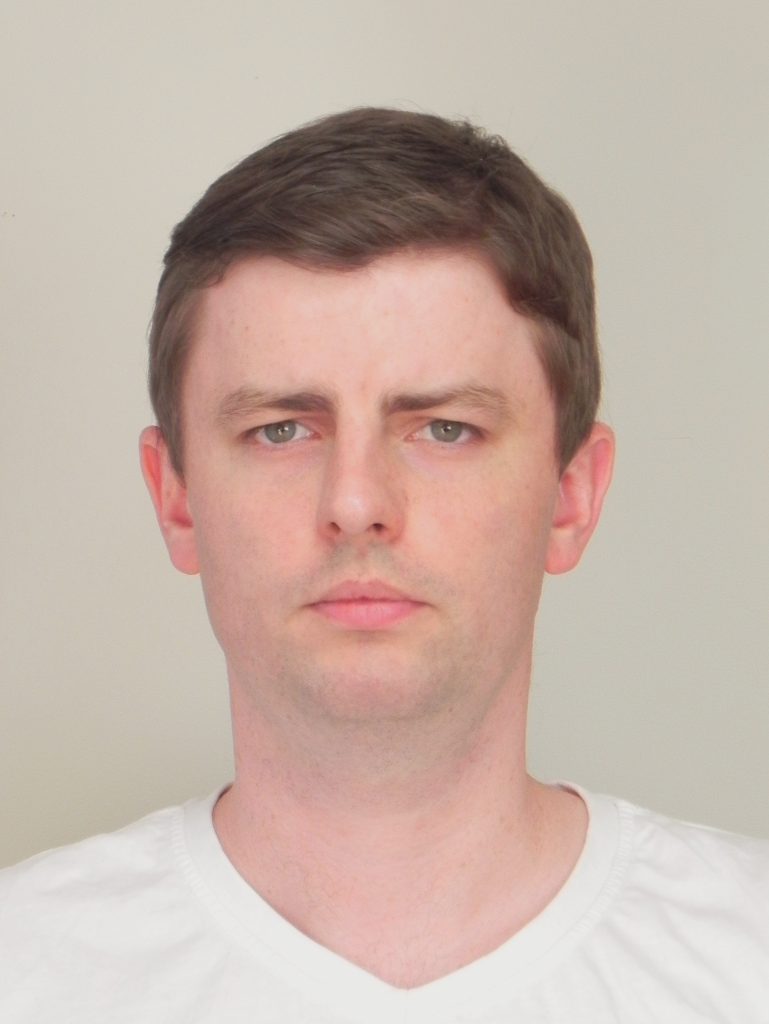
\includegraphics[width=1in,height=1.25in,clip,keepaspectratio]{graphics/MarkJones-Aug13.png}}]{Mark Jones}
received the B.Sc. degree in Physics in 2008 and the M.E. degree in Microwave Electronics in 2009 from The University of Waikato, Hamilton, New Zealand.
He is working towards a Ph.D. in Electrical Engineering, also at The University of Waikato.
\end{IEEEbiography}

\begin{IEEEbiography}[{
\includegraphics[width=1in,height=1.25in,clip,keepaspectratio]{graphics/JBSatNICTA.png}}]{Jonathan Scott}
(M'80--SM'99) is the Foundation Professor in
Electronic Engineering at the University of Waikato in Hamilton, New
Zealand.  From 1998 to 2006 he was with the Hewlett-Packard,
now Agilent Technologies, Microwave Technology Center in Santa Rosa,
where he was responsible for advanced measurement systems.  In 1997 and
1998 he was Chief Engineer at RF Technology in Sydney.  He was with The
University of Sydney in the Department of Electrical Engineering prior
to 1997.  He is a Professorial Fellow of Macquarie
University.  Professor Scott has authored over 100 refereed
publications and holds a number of patents.
\end{IEEEbiography}

\end{document}
